\documentclass{article}
\usepackage[margin=1in]{geometry}
\usepackage{amsmath}
\usepackage{amssymb}
\usepackage{graphicx}
\usepackage{mathtools}
\usepackage{tikz}
\usepackage{enumitem}
\graphicspath{images/}

\newcommand{\R}{\mathbb{R}}
\newcommand{\abs}[1]{\left\vert #1 \right\vert}

\begin{document}

\title{Piecewise Polynomials with Bounded Derivatives}
\author{Aresh Pourkavoos}
\maketitle

I originally encountered this problem on my high school robotics team.
We wanted to program a routine for our robot
to move from one point to another in a straight line in the minimum time $T$.
For simplicity, assume the robot
is moving in one dimension by a distance $d_0 > 0$.
The robot has a top speed $d_1 > 0$,
so the most straightforward routine is
to calculate the time it takes to travel the desired distance at top speed
(i.e. $T=\frac{d_1}{d_0}$)
and to run the motors for that length of time.
The velocity and position graphs for this routine are below.
\begin{center}
  \begin{tikzpicture}[scale=0.5]
    \begin{scope}[shift={(0,0)}]
      \draw[->] (-1.5, 0) -- (4.5, 0) node[right] {$t$};
      \draw[->] (0, -0.5) -- (0, 6.5) node[above] {$v$};
      \draw (0.25, 2) -- (-0.25, 2) node[left] {$d_1$};
      \draw (3, 0.25) -- (3, -0.25) node[below] {$T$};
      \draw[very thick, color=red] plot coordinates {(-1, 0) (0, 0) (0, 2) (3, 2) (3, 0) (4, 0)};
    \end{scope}
    \begin{scope}[shift={(8,0)}]
      \draw[->] (-1.5, 0) -- (4.5, 0) node[right] {$t$};
      \draw[->] (0, -0.5) -- (0, 6.5) node[above] {$x$};
      \draw (0.25, 6) -- (-0.25, 6) node[left] {$d_0$};
      \draw (3, 0.25) -- (3, -0.25) node[below] {$T$};
      \draw[very thick, color=red] plot coordinates {(-1, 0) (0, 0) (3, 6) (4, 6)};
    \end{scope}
  \end{tikzpicture}
\end{center}
However, this solution was unsatisfactory
because of the sudden acceleration from rest to top speed,
which would cause the wheels to slip
and the distance traveled to be inconsistent.
So we placed a limit $d_2 > 0$ on the acceleration,
had the robot accelerate at that rate to top speed,
maintain that speed for as long as possible,
then slow down to rest as it approached the destination.
The new graphs of acceleration, velocity, and position were:
\begin{center}
  \begin{tikzpicture}[scale=0.5]
    \begin{scope}[shift={(0,0)}]
      \draw[->] (-1.5, 0) -- (5.5, 0) node[right] {$t$};
      \draw[->] (0, -2.5) -- (0, 6.5) node[above] {$a$};
      \draw (0.25, 2) -- (-0.25, 2) node[left] {$d_2$};
      \draw (4, -0.25) -- (4, 0.25) node[above] {$T$};
      \draw[very thick, color=red] plot coordinates {(-1, 0) (0, 0) (0, 2) (1, 2) (1, 0) (3, 0) (3, -2) (4, -2) (4, 0) (5, 0)};
    \end{scope}
    \begin{scope}[shift={(9,0)}]
      \draw[->] (-1.5, 0) -- (5.5, 0) node[right] {$t$};
      \draw[->] (0, -2.5) -- (0, 6.5) node[above] {$v$};
      \draw (0.25, 2) -- (-0.25, 2) node[left] {$d_1$};
      \draw (4, 0.25) -- (4, -0.25) node[below] {$T$};
      \draw[very thick, color=red] plot coordinates {(-1, 0) (0, 0) (1, 2) (3, 2) (4, 0) (5, 0)};
    \end{scope}
    \begin{scope}[shift={(18,0)}]
      \draw[->] (-1.5, 0) -- (5.5, 0) node[right] {$t$};
      \draw[->] (0, -2.5) -- (0, 6.5) node[above] {$x$};
      \draw (0.25, 6) -- (-0.25, 6) node[left] {$d_0$};
      \draw (4, 0.25) -- (4, -0.25) node[below] {$T$};
      \draw[very thick, color=red] plot coordinates {(-1, 0) (0, 0)};
      \draw[very thick, color=red, domain=0:1] plot (\x, \x*\x);
      \draw[very thick, color=red] plot coordinates {(1, 1) (3, 5)};
      \draw[very thick, color=red, domain=3:4] plot (\x, -10+8*\x-\x*\x);
      \draw[very thick, color=red] plot coordinates {(4, 6) (5, 6)};
    \end{scope}
  \end{tikzpicture}
\end{center}
However, over short enough distances,
the robot would not have enough time to reach full speed,
so it would need to begin decelerating before then:
\begin{center}
  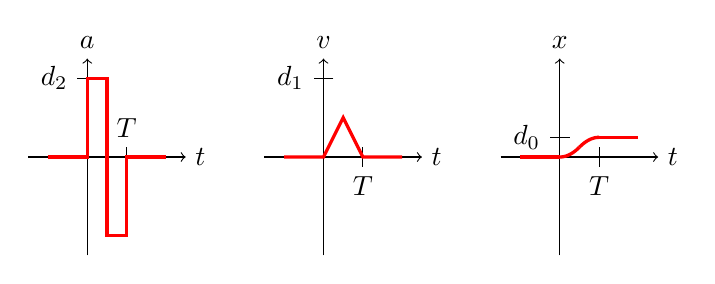
\begin{tikzpicture}[scale=0.5]
    \begin{scope}[shift={(0,0)}]
      \draw[->] (-1.5, 0) -- (2.5, 0) node[right] {$t$};
      \draw[->] (0, -2.5) -- (0, 2.5) node[above] {$a$};
      \draw (0.25, 2) -- (-0.25, 2) node[left] {$d_2$};
      \draw (1, -0.25) -- (1, 0.25) node[above] {$T$};
      \draw[very thick, color=red] plot coordinates {(-1, 0) (0, 0) (0, 2) (0.5, 2) (0.5, -2) (1, -2) (1, 0) (2, 0)};
    \end{scope}
    \begin{scope}[shift={(6,0)}]
      \draw[->] (-1.5, 0) -- (2.5, 0) node[right] {$t$};
      \draw[->] (0, -2.5) -- (0, 2.5) node[above] {$v$};
      \draw (0.25, 2) -- (-0.25, 2) node[left] {$d_1$};
      \draw (1, 0.25) -- (1, -0.25) node[below] {$T$};
      \draw[very thick, color=red] plot coordinates {(-1, 0) (0, 0) (0.5, 1) (1, 0) (2, 0)};
    \end{scope}
    \begin{scope}[shift={(12,0)}]
      \draw[->] (-1.5, 0) -- (2.5, 0) node[right] {$t$};
      \draw[->] (0, -2.5) -- (0, 2.5) node[above] {$x$};
      \draw (0.25, 0.5) -- (-0.25, 0.5) node[left] {$d_0$};
      \draw (1, 0.25) -- (1, -0.25) node[below] {$T$};
      \draw[very thick, color=red] plot coordinates {(-1, 0) (0, 0)};
      \draw[very thick, color=red, domain=0:0.5] plot (\x, \x*\x);
      \draw[very thick, color=red, domain=0.5:1] plot (\x, -0.5+2*\x-\x*\x);
      \draw[very thick, color=red] plot coordinates {(1, 0.5) (2, 0.5)};
    \end{scope}
  \end{tikzpicture}
\end{center}

$T$ still represents the total time to excecute the maneuver,
but its formula has changed.
The time to accelerate to top speed is given by $\frac{d_1}{d_2}$,
and the distance the robot travels in that time is
$\frac{d_2}{2}\left(\frac{d_1}{d_2}\right)^2=\frac{d_1^2}{2d_2}$.
If the total distance traveled is at least twice that,
i.e. if $d_0 \geq \frac{d_1^2}{d_2}$,
then the robot can reach top speed on the way.
Thus it spends $\frac{2d_1}{d_2}$ time accelerating and decelerating (altogether),
and the distance it covers at top speed is $d_0-\frac{d_1^2}{d_2}$, which takes
$\frac{1}{d_1}\left(d_0-\frac{d_1^2}{d_2}\right)=\frac{d_0}{d_1}-\frac{d_1}{d_2}$ time.
Then $T=\frac{2d_1}{d_2}+\frac{d_0}{d_1}-\frac{d_1}{d_2}=\frac{d_0}{d_1}+\frac{d_1}{d_2}$.
On the other hand, if $d_0 < \frac{d_1^2}{d_2}$,
the robot can only accelerate until it is halfway to the destination,
which also takes half of the total time
(as the other half is spent slowing back down).
Thus $\frac{d_0}{2}=\frac{d_2}{2}\left(\frac{T}{2}\right)^2$,
so $T=2\sqrt{\frac{d_0}{d_2}}$.

This solution worked well enough for our robot,
but some applications also place a limit $d_3 > 0$ on jerk,
which is the third derivative of position with respect to time,
i.e. the rate of change of acceleration.
For example, people in elevators feel acceleration as weight,
so if the elevator jumps from rest to some nonzero acceleration,
the passengers will feel a sudden weight change.
As a result, the path of an elevator
may have up to 7 polynomial pieces
(not including the phases of rest at the beginning and end).
Example jerk, acceleration, velocity, and position curves
are shown below.

\begin{center}
  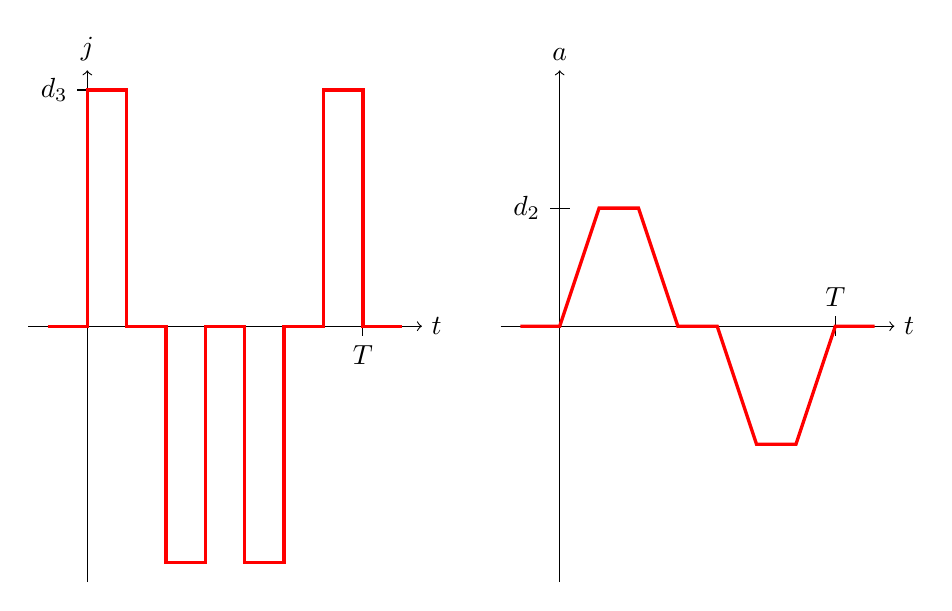
\begin{tikzpicture}[xscale=0.5,yscale=0.0625]
    \begin{scope}[shift={(0,0)}]
      \draw[->] (-1.5, 0) -- (8.5, 0) node[right] {$t$};
      \draw[->] (0, -52) -- (0, 52) node[above] {$j$};
      \draw (0.25, 48) -- (-0.25, 48) node[left] {$d_3$};
      \draw (7, 2) -- (7, -2) node[below] {$T$};
      \draw[very thick, color=red] plot coordinates {(-1, 0) (0, 0) (0, 48) (1, 48) (1, 0) (2, 0) (2, -48) (3, -48) (3, 0) (4, 0) (4, -48) (5, -48) (5, 0) (6, 0) (6, 48) (7, 48) (7, 0) (8, 0)};
    \end{scope}
    \begin{scope}[shift={(12,0)}]
      \draw[->] (-1.5, 0) -- (8.5, 0) node[right] {$t$};
      \draw[->] (0, -52) -- (0, 52) node[above] {$a$};
      \draw (0.25, 24) -- (-0.25, 24) node[left] {$d_2$};
      \draw (7, -2) -- (7, 2) node[above] {$T$};
      \draw[very thick, color=red] plot coordinates {(-1, 0) (0, 0) (1, 24) (2, 24) (3, 0) (4, 0) (5, -24) (6, -24) (7, 0) (8, 0)};
    \end{scope}
  \end{tikzpicture} \\
  \vspace{5mm}
  \begin{tikzpicture}[xscale=0.5,yscale=0.0625]
    \begin{scope}[shift={(0,0)}]
      \draw[->] (-1.5, 0) -- (8.5, 0) node[right] {$t$};
      \draw[->] (0, -4) -- (0, 52) node[above] {$v$};
      \draw (0.25, 24) -- (-0.25, 24) node[left] {$d_1$};
      \draw (7, 2) -- (7, -2) node[below] {$T$};
      \draw[very thick, color=red] plot coordinates {(-1, 0) (0, 0)};
      \draw[very thick, color=red, domain=0:1] plot (\x, 6*\x*\x);
      \draw[very thick, color=red] plot coordinates {(1, 6) (2, 18)};
      \draw[very thick, color=red, domain=2:3] plot (\x, -6*\x*\x+36*\x-30);
      \draw[very thick, color=red] plot coordinates {(3, 24) (4, 24)};
      \draw[very thick, color=red, domain=4:5] plot (\x, -6*\x*\x+48*\x-72);
      \draw[very thick, color=red] plot coordinates {(5, 18) (6, 6)};
      \draw[very thick, color=red, domain=6:7] plot (\x, 6*\x*\x-84*\x+294);
      \draw[very thick, color=red] plot coordinates {(7, 0) (8, 0)};
    \end{scope}
    \begin{scope}[shift={(12,0)}]
      \draw[->] (-1.5, 0) -- (8.5, 0) node[right] {$t$};
      \draw[->] (0, -4) -- (0, 52) node[above] {$x$};
      \draw (0.25, 48) -- (-0.25, 48) node[left] {$d_0$};
      \draw (7, 2) -- (7, -2) node[below] {$T$};
      \draw[very thick, color=red] plot coordinates {(-1, 0) (0, 0)};
      \draw[very thick, color=red, domain=0:1] plot (\x, \x*\x*\x);
      \draw[very thick, color=red, domain=1:2] plot (\x, 3*\x*\x-3*\x+1);
      \draw[very thick, color=red, domain=2:3] plot (\x, -\x*\x*\x+9*\x*\x-15*\x+9);
      \draw[very thick, color=red] plot coordinates {(3, 18) (4, 30)};
      \draw[very thick, color=red, domain=4:5] plot (\x, -\x*\x*\x+12*\x*\x-36*\x+46);
      \draw[very thick, color=red, domain=5:6] plot (\x, -3*\x*\x+39*\x-79);
      \draw[very thick, color=red, domain=6:7] plot (\x, \x*\x*\x-21*\x*\x+147*\x-295);
      \draw[very thick, color=red] plot coordinates {(7, 48) (8, 48)};
    \end{scope}
  \end{tikzpicture}
\end{center}

At this point, the general version of the problem begins to suggest itself.
Given an integer $n \geq 1$ and positive real numbers $d_0, d_1, \ldots, d_n$,
the task is to find a function $x : \R \rightarrow \R$ where

\begin{enumerate}
\item
  $x(t)=0$ for all $t \leq 0$;
\item
  $x(t)=d_0$ for all $t \geq T$, where $T > 0$;
\item
  $\abs{x^{(i)}(t)} \leq d_i$
  for all $t \in \R$ and $i \in \{1, \ldots, n\}$
  where $x^{(i)}(t)$ denotes the $i^\text{th}$ derivative of $x$ at $t$;
\item
  the value of $T$ is minimized among all functions
  which satisfy properties 1-3.
\end{enumerate}

Actually, the problem statement above is slightly inaccurate,
specifically property 3,
as the $n^\text{th}$ derivative is not defined everywhere.
In the figure above, there are $8$ transition points between the phases.
At these points, the acceleration $a = x^{(n-1)}$ has no derivative,
so the jerk is undefined.
Instead of saying that the derivative of $x^{(n-1)}$
(i.e. $j = x^{(n)}$) must be bounded by $d_n$,
we say that $x^{(n-1)}$ must be \textit{Lipschitz continuous}
with Lipschitz constant $d_n$.
This means that
\[
\abs{\frac{x^{(n-1)}(t_2)-x^{(n-1)}(t_1)}{t_2-t_1}} \leq d_n
\]
for all $t_1, t_2 \in \R$.
Geometrically speaking, this is equivalent to
every \textit{secant} line of the graph of $x^{(n-1)}$
having a slope between $-d_n$ and $d_n$
(rather than every \textit{tangent} line as bounding $x^{(n)}$ would suggest).
So property 3 may be more accurately written as
\begin{enumerate}
  \setcounter{enumi}{2}
\item
  $\abs{x^{(i)}(t)} \leq d_i$
  for all $t \in \R$ and $i \in \{1, \ldots, n-1\}$,
  and $x^{(n-1)}$ has Lipschitz constant $d_n$.
\end{enumerate}

I have not yet been able to solve this problem in full,
but I have done three things:
\begin{enumerate}
  \item
    Find an algorithm to produce \textit{a} function
    which satisfies properties 1-3 for any values of $d_0, \ldots, d_n$.
    However, this is not \textit{the} function which minimizes $T$.
  \item
    Find the (probably) optimal solution
    in the case where $x^{(n-1)}$ has Lipschitz constant $d_n$,
    but $\abs{x^{(i)}}$ is not restricted for $i \in \{1, \ldots, n-1\}$.
    Equivalently, this is the case where $d_1, \ldots, d_{n-1}$ are very large,
    so $d_n$ is the only ``bottleneck.''
  \item
    Combine the previous two cases in a nontrivial way
    to take advantage of both of their strengths.
    This approach
    \begin{itemize}
    \item
      returns a solution for any values of $d_0, \ldots, d_n$
      (which is at least as good as that of case 1);
    \item
      returns the same thing as case 2 whenever the latter is applicable;
    \item
      and (this is the nontrivial part)
      sometimes returns a solution \textit{better} than that of case 1,
      even when case 2 is \textit{not} directly applicable.
    \end{itemize}
\end{enumerate}
The algorithm in case 1 arose from the following observation:
the velocity graph for $n=2$
looks like two reflected copies of the position graph for $n=1$,
separated by a constant function at $d_1$.
Likewise, the velocity graph for $n=3$
looks like two reflected copies of the position graph for $n=2$,
separated by a constant function at $d_1$.  
In general, this makes sense:
in order to get from $0$ to $d_0$ with $n$ derivatives restricted,
the velocity needs to increase from $0$ to $d_1$ (or less),
stay at the maximum for some length of time (possibly $0$ time),
and then decrease back to $0$.
But the increasing portion of the velocity
may be seen as a smaller instance of the same problem,
where the first $n-1$ derivatives are restricted rather than $n$,
and the decreasing portion is a mirror image of that.
The base case $n=1$, as seen above, is just a straight line segment.

\end{document}
